\documentclass{beamer}

\mode<presentation> {
\usetheme{Boadilla} % Singapore
\usecolortheme{beaver}
}

\usepackage{graphicx} % Allows including images
\usepackage{booktabs} % Allows the use of \toprule, \midrule and \bottomrule in tables
\usepackage{amsmath}
\usepackage{amsfonts}
\usepackage{ifthen}
\usepackage{amssymb}
\usepackage{amsbsy}
\usepackage{bm}
\usepackage{multicol}
\usepackage{ulem}
\usepackage{float}
\usepackage{latexsym}
\usepackage{comment}
\usepackage{graphicx}
\usepackage{amstext}
\usepackage{latexsym}
\usepackage{arydshln}
\usepackage{longtable}
\usepackage{enumerate}
\usepackage{multirow}
\usepackage{cases}
\usepackage{geometry}
\usepackage{mathtools}
\usepackage{subeqnarray}
\usepackage{textcomp}
\usepackage{hyperref}
%\usepackage{subfigure}
\usepackage{url}
\usepackage{threeparttable}
\usepackage{xr}
\usepackage{multirow}
\usepackage{wrapfig}
\usepackage{lscape}
\usepackage{rotating}
\usepackage{subcaption}
\usepackage{epstopdf}
\usepackage{verbatim}
\usepackage{dsfont}
\usepackage[sort&compress]{natbib}
\setbeamertemplate{theorems}[numbered]
\newtheorem{prop}{Proposition}
\let\oldframe\frame
\renewcommand{\frame}{%
\oldframe
\let\olditemize\itemize
\renewcommand\itemize{\olditemize\addtolength{\itemsep}{10pt}}%
}
\def\mathbf#1{\textbf{\em #1}}
\newcommand{\qvec}[1]{\textbf{\textit{#1}}}
%\newtheorem{theorem}{Theorem}
%\newtheorem{lemma}{Lemma}
\newtheorem{proposition}[theorem]{Proposition}
%\newtheorem{corollary}[theorem]{Corollary}
%\newtheorem{definition}{Definition}
\newtheorem{assumption}{Assumption}
%\newenvironment{proof}{{\bf Sketch of proof:}}{\hfill\rule{2mm}{2mm}}
\newcommand{\Ep}{\mathbb{E}^P}
\newcommand{\bX}{\boldsymbol{X}}
\newcommand{\bzero}{\boldsymbol{0}}
\newcommand{\btheta}{\boldsymbol{\theta}}
\newcommand{\bpsi}{\boldsymbol{\psi}}
\newcommand{\bg}{\boldsymbol{g}}
\newcommand{\bv}{\boldsymbol{v}}
\newcommand{\bx}{\boldsymbol{x}}

\definecolor{darkgreen}{RGB}{34,139,34}
\definecolor{darkred}{RGB}{200, 16, 26}

%----------------------------------------------------------------------------------------
%	TITLE PAGE
%----------------------------------------------------------------------------------------


\title[ISU team 2]{%
2019 Data Mining Cup Best Solution}

\author[]{
	Qihao Zhang, Yifan Zhu, Xingche Guo
}
\institute[Dept. of Statistics, ISU]{Department of Statistics, Iowa State University}
\date{\today}

\AtBeginSection[]{
	\begin{frame}
	\vfill
	\centering
	\begin{beamercolorbox}[sep=8pt,center,shadow=true,rounded=true]{title}
		\usebeamerfont{title}\insertsectionhead\par%
	\end{beamercolorbox}
	\vfill
\end{frame}
}

\begin{document}
\begin{frame}
\titlepage
\end{frame}

\begin{frame}
\frametitle{Table of Contents}
\tableofcontents
\end{frame}


%%%%%%%%%%%%%%%%%%%%%%%%%%%%%%%%%%%%%%%
\section{Problem Introduction and Data Description}
\begin{frame}
\frametitle{Scenario}
\begin{itemize}
    \item \textbf{Data}: A self-checkouts data in retail collecting by handheld scanners
    \item \textbf{Domain Knowledge}: Approximate 5\% discrepancy
    \item \textbf{Discrepancy}: Intentionally, or accidentally, or machine problem
    \item \textbf{Task}: Classify a half million scans in the test set as fraudulent or not fraudulent by building up a model on the training set
    \item \textbf{Evaluation}: Achieve the highest monetary profit on the test set
    
\end{itemize}
\end{frame}

\begin{frame}
\frametitle{Features}
    \small{
\begin{table}[H]
    \centering
    \begin{tabular}{|c|c|p{52mm}|}
    \hline
        1 & TrustLevel & How trustworthy \\ \hline
        2 & totalScanTimeInSeconds & How long for purchasing (Seconds)\\ \hline
        3 & grandTotal & How much spent (\$)\\ \hline
        
        4* & lineItemVoids & number times of Void Scanning \\ \hline 
        5* & scansWithoutRegistration & number times of Invalid Scanning \\ \hline
        6 & quantityModification & number times of error but legitimate scanning  \\ \hline
        7** & scannedLineitemsPerSeconds & How fast of scanning (item/second)   10/2 \\ \hline
        8** & valuePerSecond & How fast of scanning (\$/second)       3/2 \\ \hline
        9** & lineItemVoidPerPosition & Void Scanning/Legitimate Scanning   4/10  \\ \hline
        10* & itemTotal (New feature) & number times of Legitimate Scanning (total items) (Manually made 2\times 7)\\ \hline
        11 & fraud (Response) &   fraud or not fraud (1 or 0) \\ \hline
    \end{tabular}
\end{table}
}
\end{frame}

\begin{frame}
\frametitle{Training Set}
    \begin{itemize}
        \item Total 1879 scan observations and 9 original features
        \item 104 (5.5\%) samples are frauds and 1775 (94.5\%) samples are no frauds
        \item Denote fraud as 1 and no fraud as 0
        \item No fraud in the training set with TrustLevel 3, 4, 5, 6
    \end{itemize}
\end{frame}

\begin{frame}
\frametitle{Conditional Empirical Distribution $\hat{f}(x|y)$}
\begin{figure}[H]
		\centering
		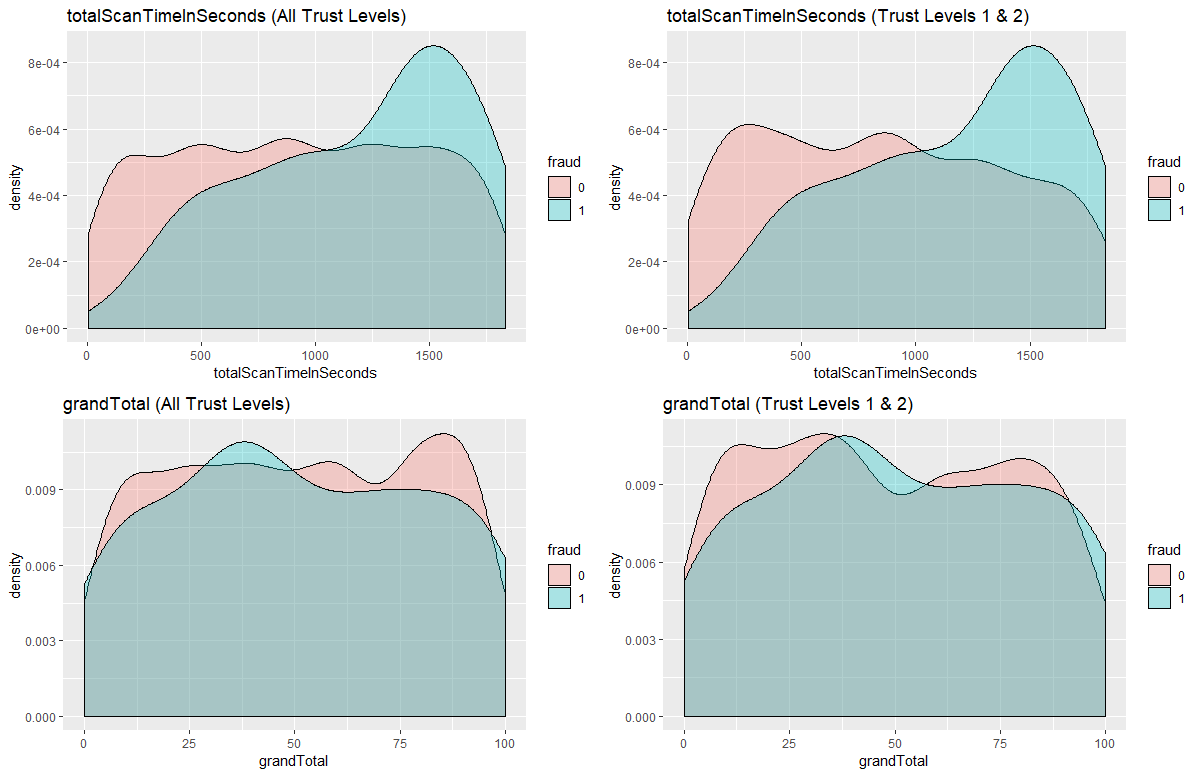
\includegraphics[width = 0.9\textwidth]{figure/DATA_P1.png}
	\end{figure}
\end{frame}

\begin{frame}
\frametitle{Conditional Empirical Distribution $\hat{f}(x|y)$}
\begin{figure}[H]
		\centering
		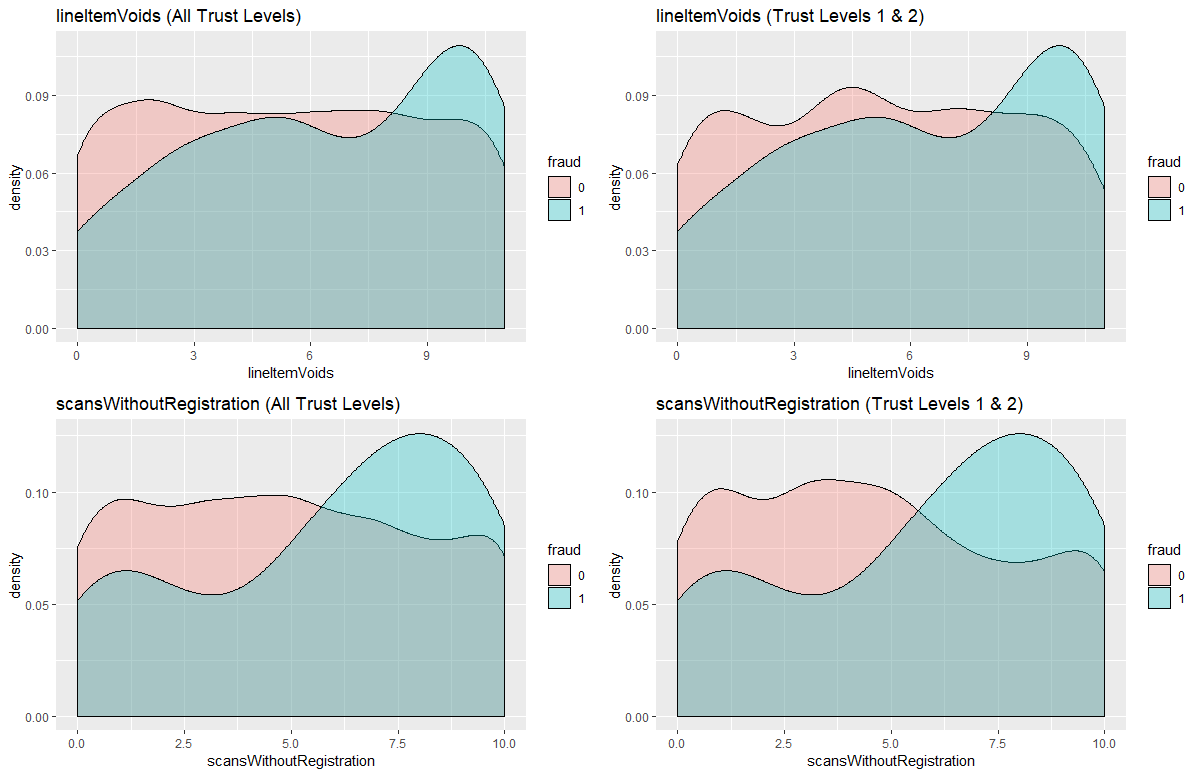
\includegraphics[width = 0.9\textwidth]{figure/DATA_P2.png}
	\end{figure}
\end{frame}

\begin{frame}
\frametitle{Conditional Empirical Distribution $\hat{f}(x|y)$}
\begin{figure}[H]
		\centering
		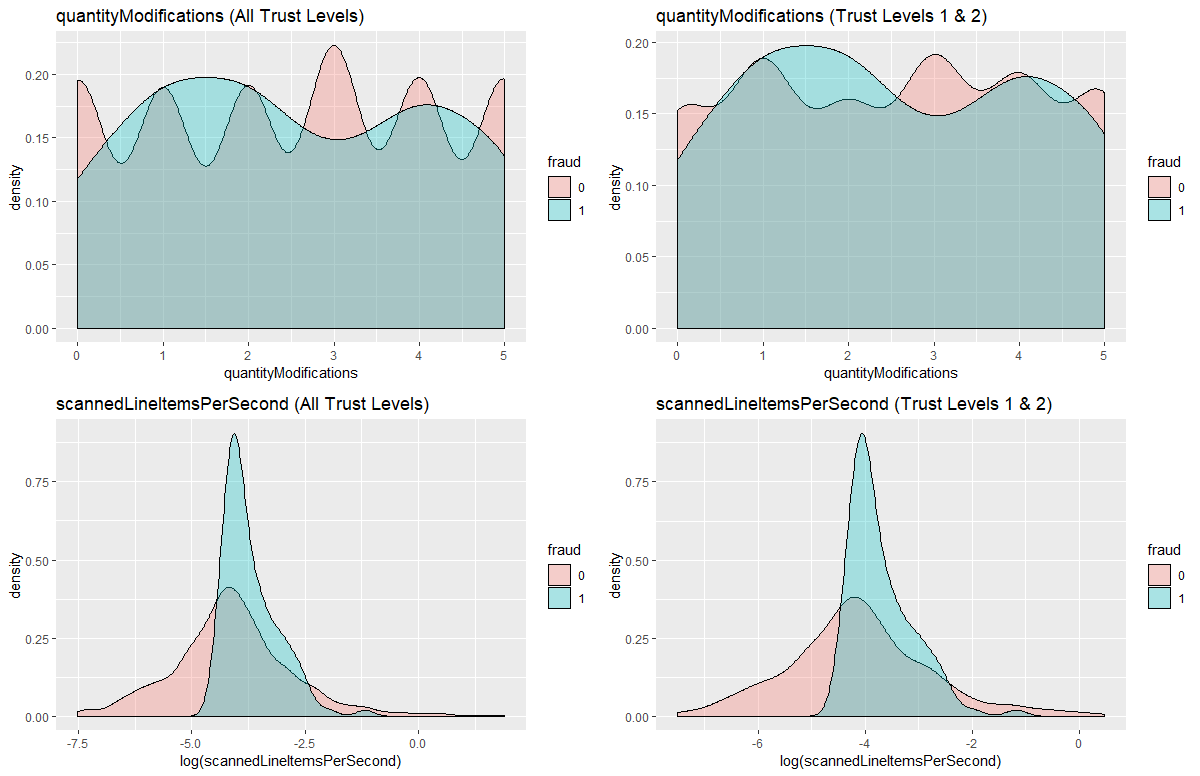
\includegraphics[width = 0.9\textwidth]{figure/DATA_P3.png}
	\end{figure}
\end{frame}

\begin{frame}
\frametitle{Conditional Empirical Distribution $\hat{f}(x|y)$}
\begin{figure}[H]
		\centering
		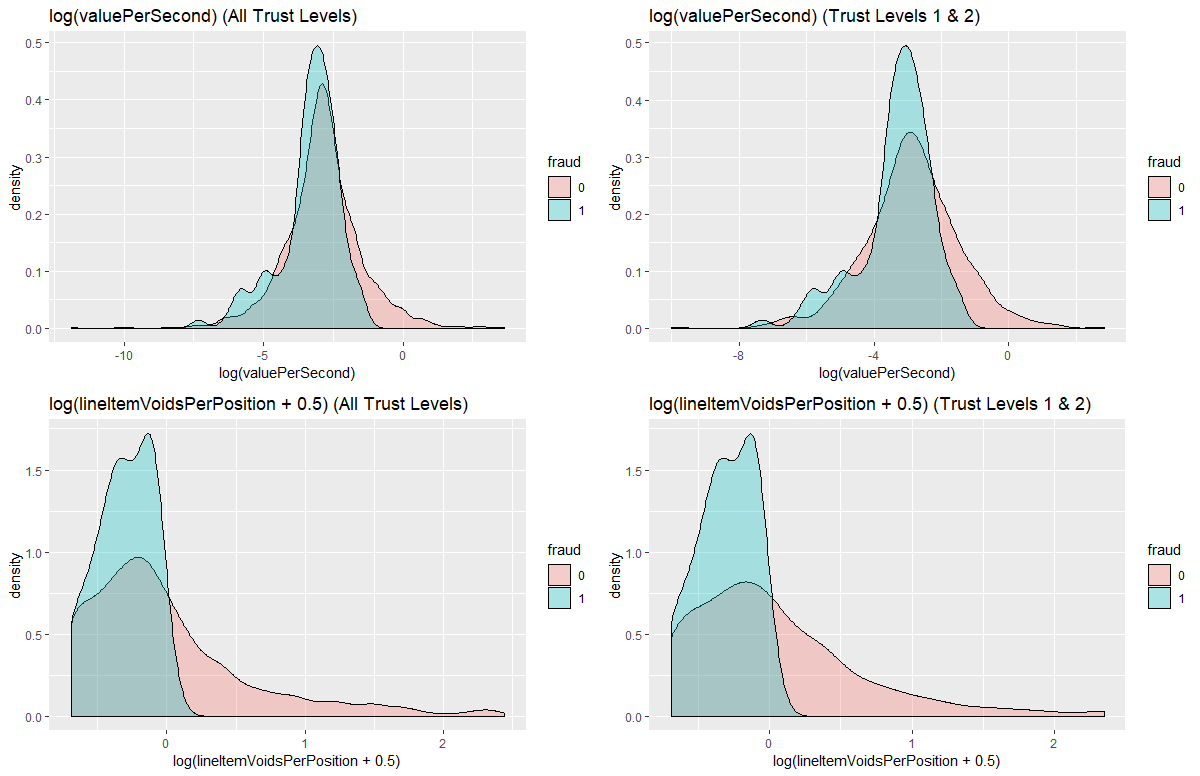
\includegraphics[width = 0.9\textwidth]{figure/DATA_P4.png}
	\end{figure}
\end{frame}

\begin{frame}
\frametitle{Conditional Empirical Distribution $\hat{f}(x|y)$}
\begin{figure}[H]
		\centering
		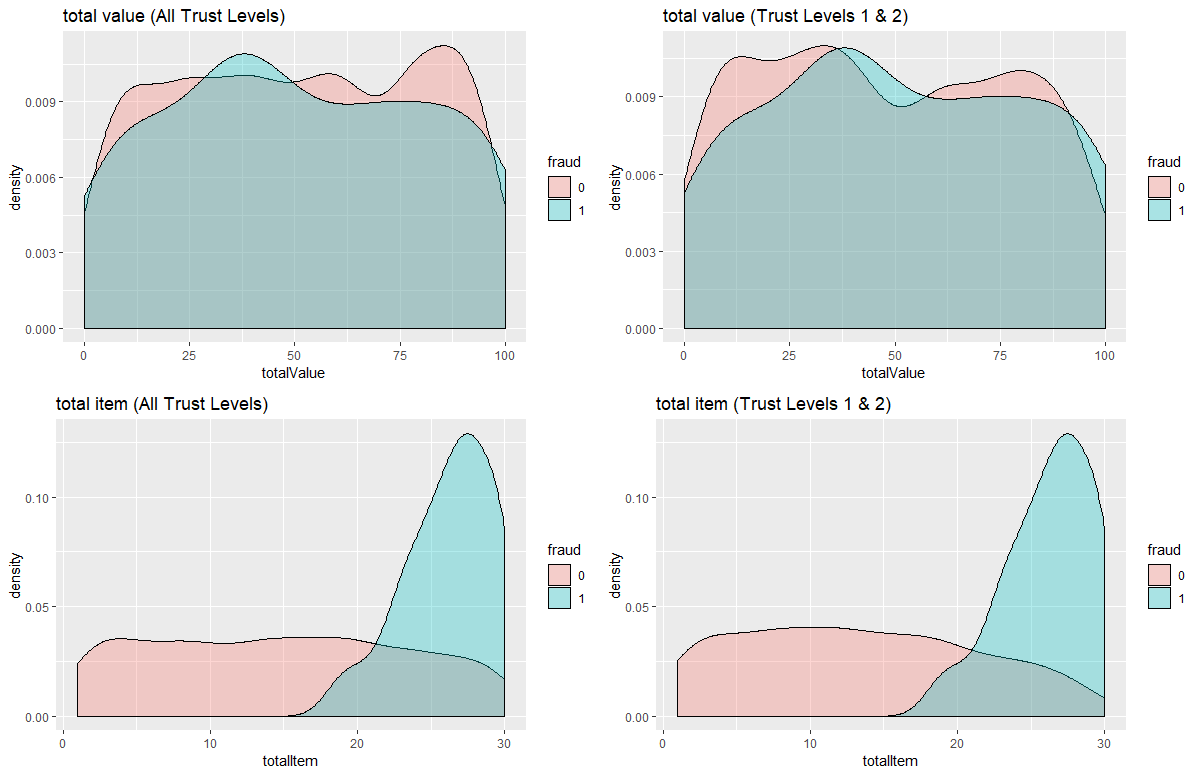
\includegraphics[width = 0.9\textwidth]{figure/DATA_P5.png}
	\end{figure}
\end{frame}

\begin{frame}
 \frametitle{Monetary Profit (Score function)}  
\begin{table}[ht]
%\begin{center}
\begin{tabular}{|c|l|l|l|}
    \hline
    \multirow{4}{*}{\textbf{Prediction}} & \multicolumn{3}{|c|}{\textbf{Actual value}}\\ \cline{2-4}
    &  & 0 (no fraud) & 1 (fraud)\\ \cline{2-4}
    & 0 (no fraud) & 0 & -5\\ \cline{2-4}
    & 1 (fraud) & -25 & 5\\ \hline
\end{tabular}
%\end{center}
\end{table}

\begin{itemize}
\item The sum of the profit or score of all scans in the testing set is the monetary value of the submitted solution.
\item We need to submit $0-1$ prediction instead of the predicted probability.
\item Score Function: \\
$S(y,\hat{y})=5 \times I(y=1,\hat{y}=1) - 5 \times I(y=1,\hat{y}=0) - 25 \times I(y=0,\hat{y}=1)$
\end{itemize}
\end{frame}

\begin{frame}
\frametitle{Modeling Procedure}
    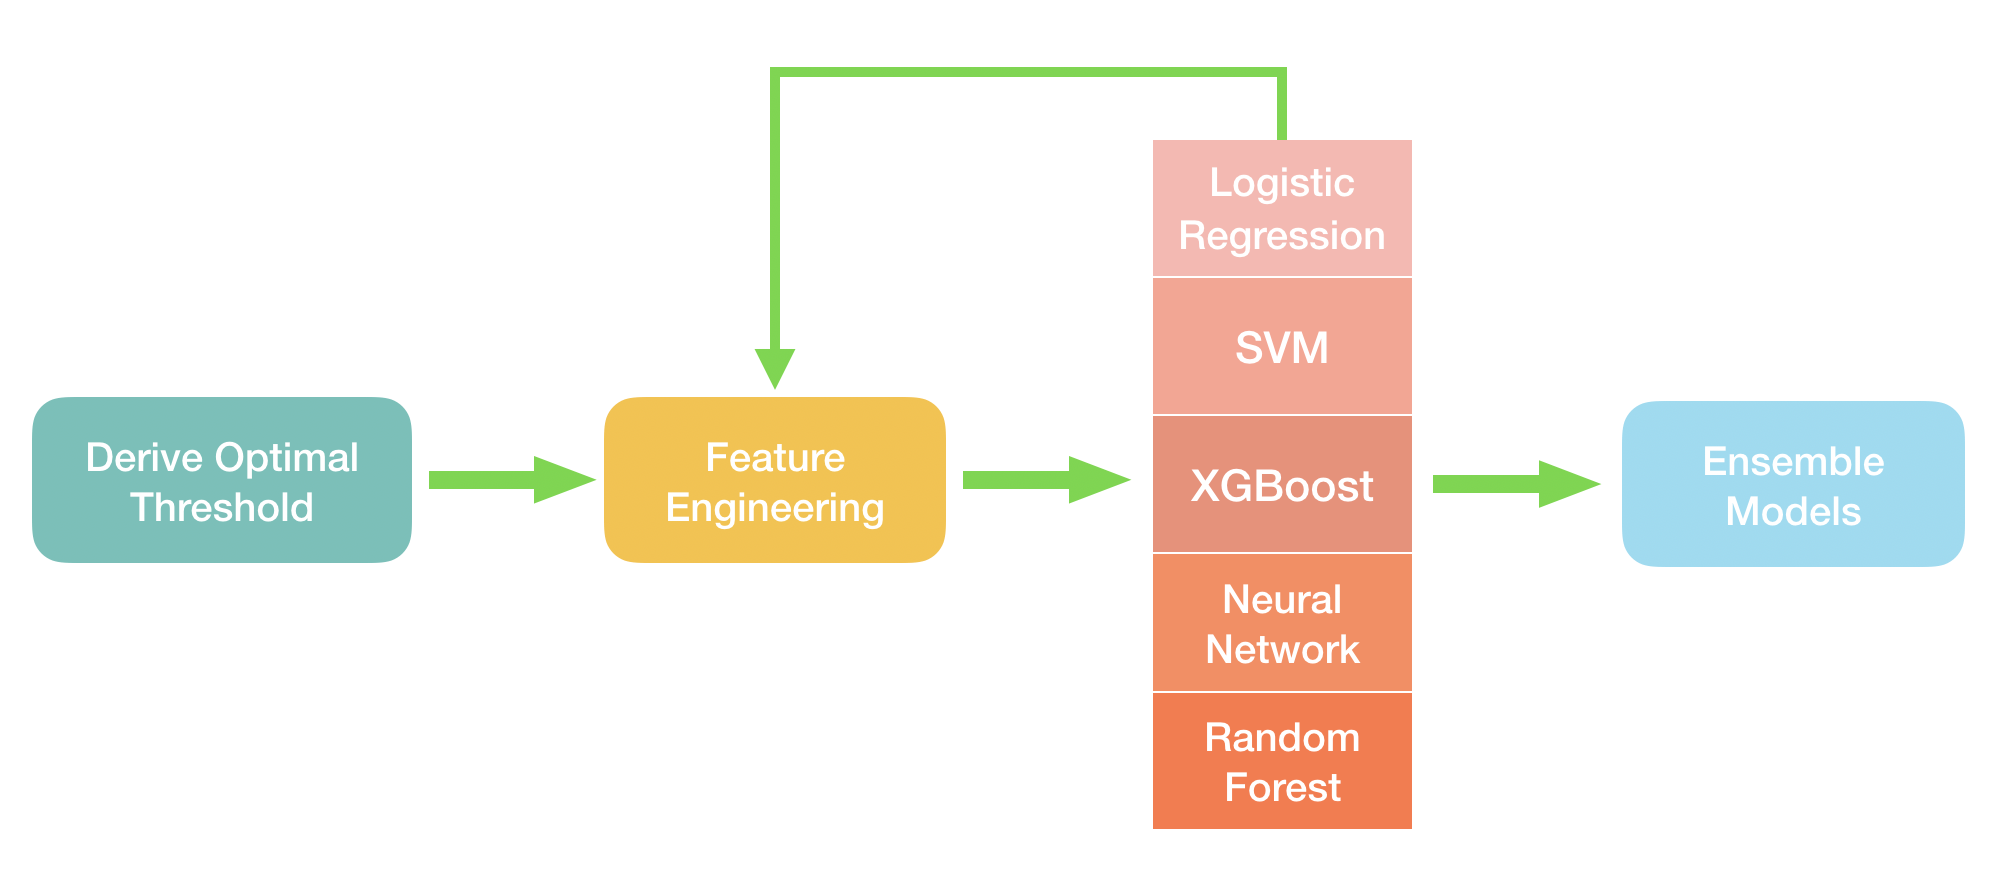
\includegraphics[width = \textwidth]{figure/FlowChart.png}
\end{frame}
%%%%%%%%%%%%%%%%%%%%%%%%%%%%%%%
\section{Evaluation Criteria and Cross-Validation Design}



\begin{frame}
\frametitle{{Loss Function and the Optimal Threshold}}
    \begin{itemize}
        \item 
        An unbalanced loss is given by the negative of the score function in this problem. Therefore we need an optimal decision rule for this loss. 
        \item  Let $y$ and $\hat{y}$ be the truth and prediction and $\bm x$ be the vector of features. 
        \item Denote $L(y, \hat{y}) = - S(y, \hat{y})$ as the loss function in this contest,  we predict $\hat{y}=1$ when: 
  $$\mathbb{E}[{L}({y}, 1) | \bm{x}]<\mathbb{E}[{L}({y}, 0) | \bm{x}],$$
By solving the inequality, we have:
$$
{p}(1 | \bm {x})>\frac{{L}(0,1)-{L}(0,0)}{{L}(1,0)-{L}(0,0)-{L}(1,1)+{L}(0,1)} = \frac{5}{7}
$$
Therefore, \textbf{fraud is detected when ${\hat{p}(1|\bm x)>5/7}$}.
    
    \end{itemize}

   
    
\end{frame}

\begin{frame}
    \frametitle{The Oracle Bound}
\begin{itemize}
    \item With the optimal threshold, all the models hereby aim to find a good approximation of the conditional probability $\hat{p}(1|\bm x)$.
    \item For this training data set, we have 104 fraud “1” out of 1879 data points. Since we cannot classify every customer correctly as fraud or no fraud , then oracle upper bound of total score (when all are classified correctly) for this training data is
    \[\sum_{i=1}^n S(y_i, \hat{y}_i) = 5 \times 104 = 520\]
\end{itemize}
\end{frame}

\begin{frame}
\frametitle{Model Performance Evaluation}
\begin{itemize}
    \item We use repeated cross-validation to evaluate the prediction ability of the models.
    \item For each repetition:
    \begin{enumerate}
        \item Shuffle training data and split shuffled data set into k folds
        \item Fit the model using $k-1$ folds and predict on the remaining 1 fold according to the optimal threshold
        \item Calculate the score on each left-out fold
        \item Run thorough all $k$ left-out folds; add these scores and get a total score, i.e.
        \[\sum_{i=1}^n S(y_i, \hat{y}_i^{CV})\]
    \end{enumerate}
    \item We repeat the cross validation 100 times with different partitions of the dataset and obtain 100 total scores.
    A good model should give a high total score and be robust to different partitions: the mean and variability of the 100 scores are used to evaluate a model 
\end{itemize}
\end{frame}

\begin{frame}
\frametitle{Cross Validation Design}
\begin{itemize}
    \item Two ways to split the dataset:
    \begin{itemize}
        \item (Random Split) randomly split the data into $k$ folds of about the same size 
        \item (Proportional Split) split the data into $k$ folds of about the same size such that the proportion of fraud in each fold is the same as the original data
    \end{itemize}
    \item Number of folds used: $k = 5$ and $k = 10$
    \item The combination leads to 4 different designs of cross validation. Every model is evaluated under all 4 designs. 
\end{itemize}
\end{frame}

\begin{frame}
\frametitle{"Best Linear" Model}
{\small
For all subset of the original features + totalItem,  based on our evaluation criteria, the best model we have now is the logistic regression model with 6 terms:
\textcolor{blue}{
\begin{align*}
& trustLevel + totalItem + lineItemVoids + scansWithoutRegistration +\\
& totalScanTimeInSeconds + grandTotal 
\end{align*}
}

The table below shows the negative of total score (we can call it total loss) $\sum_{i=1}^n L(y, \hat{y}_i^{CV}) = - \sum_{i=1}^n S(y_i, \hat{y}_i^{CV})$.

\begin{table}[H]
\scalebox{0.9}{
\begin{tabular}{ccccccc}
\hline
 & \multicolumn{2}{c}{ Random Split CV} &  \multicolumn{2}{c}{ Proportional Split CV}   \\
 &   5 Fold &  10 Fold   &   5 Fold  &  10 Fold  \\
\hline
Mean  &  -313.05   & -309.75  &  -304.65    &-306.5    \\          
SD      &  25.3       & 19.5     &  23.7       &   18.9   \\ 
\hline
Min         & -365    & -320 &  -345   &   -365    \\ 
Q1          & -330 & -320 &   -320   &   -320    \\ 
Median   & -310    & -310 &   -310   &   -310    \\ 
Q3          & -300    & -300 &   -287.5   &   -297.5    \\ 
Max        & -235    & -240 &   -240   &   -260    \\ 
\hline
\end{tabular}
}
\end{table}
}


\end{frame}



%%%%%%%%%%%%%%%%%%%%%%%%%%%%%%%%
\section{Feature Engineering and Machine Learning Model Selection}

\begin{frame}
\frametitle{Feature Engineering}
    To find good features $x$ that can separate 0 and 1
    \begin{itemize}
        \item Conditional distributions $f(x|y=0)$ and $f(x|y=1)$ have separable domains
        \item Conditional distributions $f(x|y=0)$ and $f(x|y=1)$ have different shapes
    \end{itemize}
    For example:
    \[totalItem = scannedLineItemsPerSecond \times totalScanTimeInSeconds \]
    is an important feature made from the original features.
    
\end{frame}

\begin{frame}
        \centering
        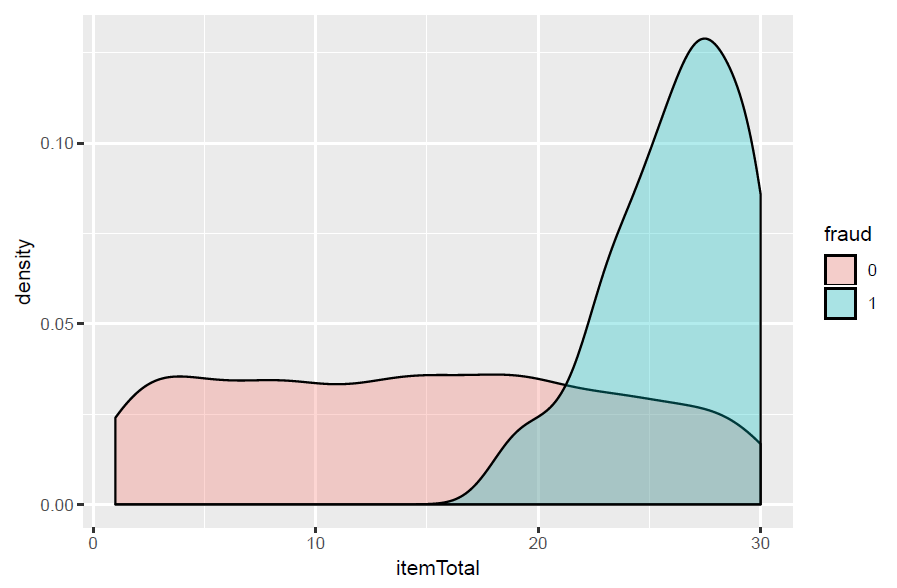
\includegraphics[width = \textwidth]{figure/TotalItem.PNG}

\end{frame}

\begin{frame}
\frametitle{Important Interaction Terms}
\begin{itemize}
\item The correlation plot matrix is made separately for all data labeled "fraud" and "no fraud".
\item Important interaction terms are added to the set of candidate features.
\end{itemize}
\end{frame}
\begin{frame}
\textbf{no fraud:}

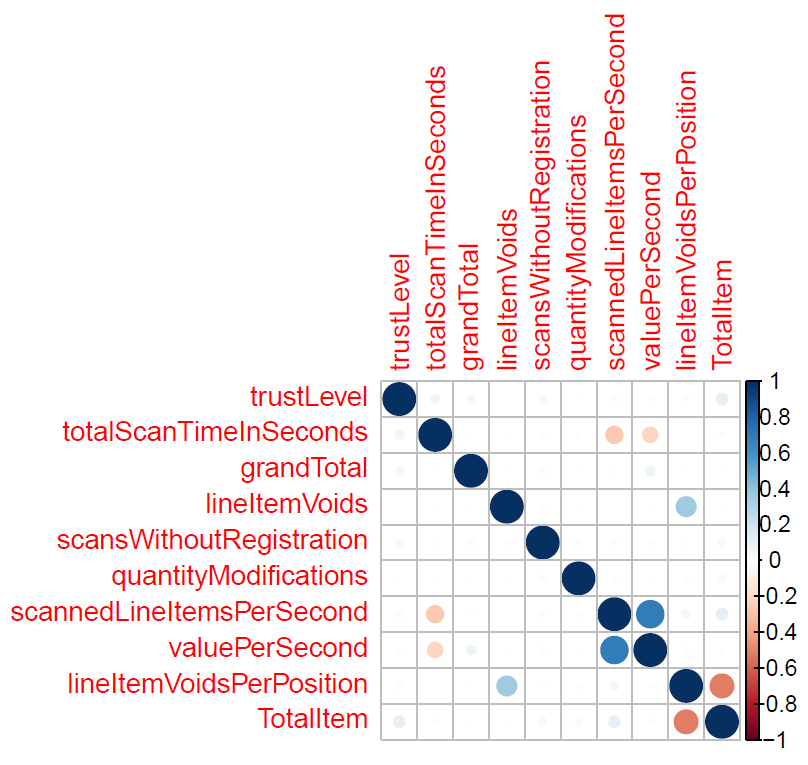
\includegraphics[width = 0.75\textwidth]{figure/corr_nofraud.PNG}
\end{frame}

\begin{frame}
\textbf{fraud:}

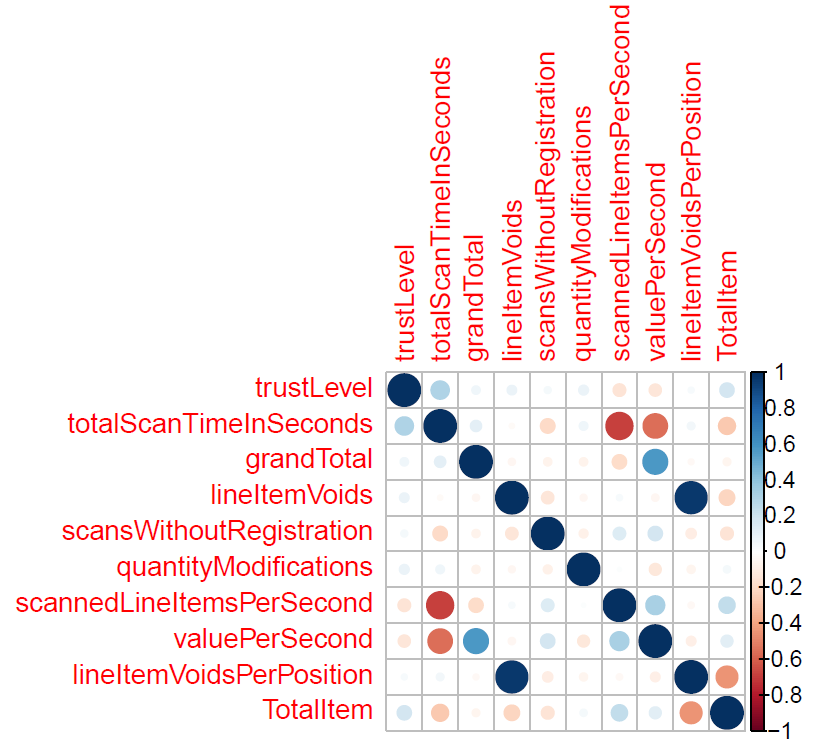
\includegraphics[width = 0.75\textwidth]{figure/corr_fraud.PNG}
\end{frame}

\begin{frame}
\frametitle{Model Selection}
\begin{itemize}
    \item Original features and potential good non-linear combination of the original features (e.g. totalItem) are added to the model
    \item Potential important interactions are added to the model
    \item Importance of features are obtained for each machine learning model, and unimportant features are removed
    \item All models are re-evaluated with only important features
    \item Logistic regression models turn to be the best using our evaluation criteria; other models tend to overfit
\end{itemize}
\end{frame}





%%%%%%%%%%%%%%%%%%%%%%%%%%%%%%%%%%
\section{The Final Method and Solutions}

\begin{frame}
\frametitle{Best Model So Far}
Our best model so far is the logistic regression model with feature set:
\textcolor{blue}{
\begin{align*}
trustLevel + totalItem + lineItemVoids + scansWithoutRegistration +\\
 totalScanTimeInSeconds + grandTotal +  grandTotal \times valuePerSecond
\end{align*}
}


\vspace{-1.5em}
\begin{table}[H]
\scalebox{0.8}{
\begin{tabular}{ccccccc}
\hline
 & \multicolumn{2}{c}{ Random Split CV} &  \multicolumn{2}{c}{ Proportional Split CV}   \\
 &   5 Fold &  10 Fold   &   5 Fold  &  10 Fold  \\
\hline
Mean  &  -311.9   & \textcolor{darkgreen}{-336.5}  &  -307.3    &\textcolor{darkgreen}{-334.7}     \\          
SD      &  \textcolor{darkred}{47.9}       & 27.5     &  \textcolor{darkred}{41.7}       &   28.6   \\ 
\hline
Min         & -395    & -385 &  -395   &   -390    \\ 
Q1          & -347.5 & -360 &   -335   &   -357.5    \\ 
Median   & -315    & -340 &   -310   &   -340    \\ 
Q3          & -285    & -325 &   -275   &   -315    \\ 
Max        & -150    & -230 &   -180   &   -260    \\ 
\hline
\end{tabular}
}
\end{table}


Compare to the best additive logistic model (with 6 additive terms), the best logistic interaction model:
\begin{itemize}
\item performs much better for 10-fold CV.
\item has \textcolor{red}{similarly mean} scores and \textcolor{red}{larger variance} for 5-fold CV.
\end{itemize}



\end{frame}







\begin{frame}
\frametitle{Further Feature Engineering}
Note that  \textcolor{red}{
$$grandTotal = totalScanTimeInSeconds \times valuePerSecond,$$}
 we can re-express the so far best model as:
\textcolor{blue}{
\begin{align*}
trustLevel + totalItem + lineItemVoids + scansWithoutRegistration +\\
 totalScanTimeInSeconds \times (1 + valuePerSecond + valuePerSecond^2)
\end{align*}
}
 Define \textcolor{red}{$V:= valuePerSecond$}; \textcolor{red}{$T:=totalScanTimeInSeconds$}; $f(V)$ to be some function of $V$. Then one possible underlying feature would be: 
 \textcolor{blue}{$$ Interaction(T,V) = T \times f(V) , $$}
where in our best logistic model so far: \textcolor{blue}{
$$  f_{(2)}(V) = 1 + V + V^2. $$}

\end{frame}



\begin{frame}
\frametitle{Further Feature Engineering}

 \textcolor{blue}{
$ f_{(4)}(V) = 1 + V + V^4. $}

\vspace{1em}
\begin{table}[H]
\scalebox{0.9}{
\begin{tabular}{ccccccc}
\hline
 & \multicolumn{2}{c}{ Random Split CV} &  \multicolumn{2}{c}{ Proportional Split CV}   \\
 &   5 Fold &  10 Fold   &   5 Fold  &  10 Fold  \\
\hline
Mean      & \textcolor{darkred}{-296.05}   & \textcolor{darkgreen}{-355.3}  &  \textcolor{darkgreen}{-316.8}    & \textcolor{darkgreen}{-349.1}     \\          
SD          & \textcolor{darkred}{242.5}       & \textcolor{darkred}{34.5}     &  \textcolor{darkred}{71.9}       &   \textcolor{darkred}{50.93}   \\ 
\hline
Min         & -420    & -420    &  -420   &   -420    \\ 
Q1          & -350    & -377.5 &   -350   &   -370    \\ 
Median   & -327.5    & -360    &   -325   &   -357.5    \\ 
Q3          & -292.5    & -335    &   -295   &   -335    \\ 
Max        & \textcolor{red}{2040}    & -215    &   110   &   65    \\ 
\hline
\end{tabular}
}
\end{table}

\vspace{1em}

Compare to $f_{(2)}(V)$, the logistic model with $f_{(4)}(V)$:
\begin{itemize}
\item performs even better for 10-fold CV.
\item performs worse for 5-fold CV.
\end{itemize}

\end{frame}





\begin{frame}
\frametitle{Further Feature Engineering}

 \textcolor{blue}{
$ f_{(log)}(V) = 1 + log(V). $}

\vspace{1em}
\begin{table}[H]
\scalebox{0.9}{
\begin{tabular}{ccccccc}
\hline
 & \multicolumn{2}{c}{ Random Split CV} &  \multicolumn{2}{c}{ Proportional Split CV}   \\
 &   5 Fold &  10 Fold   &   5 Fold  &  10 Fold  \\
\hline
Mean      & \textcolor{darkgreen}{-328.9}   & \textcolor{darkred}{-337.5}  &  \textcolor{darkgreen}{-326.6}    & \textcolor{darkred}{-339.2}     \\          
SD          & \textcolor{darkgreen}{24.4}       & \textcolor{darkgreen}{16.7}     &  \textcolor{darkgreen}{26.4}       &   \textcolor{darkgreen}{17.9}   \\ 
\hline
Min         & -375    & -365    &  -375   &   -385    \\ 
Q1          & -345    & -355    &   -345   &   -355    \\ 
Median   & -330    & -332.5 &   -330   &   -340    \\ 
Q3          & -315    & -330    &   -310   &   -330    \\ 
Max        & -230    & -295    &   -240   &   -285    \\ 
\hline
\end{tabular}
}
\end{table}

\vspace{1em}

Compare to $f_{(4)}(V)$, the logistic model with $f_{(log)}(V)$:
\begin{itemize}
\item performs much better for 5-fold CV (in terms of both mean and variance).
\end{itemize}

\end{frame}











\begin{frame}
\frametitle{ Logistic Ensemble Models }
\framesubtitle{By Probability Mixture distribution}

Define $ \hat{\mathrm{P}}(y=1 | \pmb{x}, \mathcal{F}_i)$ to be the fitted conditional probabilities by logistic regression using feature set $i$, denote $\hat{\omega}_i = \hat{\mathrm{P}}(\mathcal{F}_i)$, then:

\begin{equation*}
\hat{\mathrm{P}}^{(en)}(y=1 | \pmb{x}) = \sum_{i=1}^{d} \hat{\omega}_i  \hat{\mathrm{P}}(y=1 | \pmb{x}, \mathcal{F}_i), \ \ \ subject \ to \sum_{i=1}^d \hat{\omega}_i = 1.
\end{equation*}

\vspace{1em}

\begin{itemize}
\item The ensemble model integrates the \textcolor{red}{simple model} \textcolor{blue}{(low fitting error, high model error)} and \textcolor{red}{complex model} \textcolor{blue}{(high fitting error, low model error)}.
\item Choose proper weights such that the ensemble model has smaller \textcolor{blue}{fitting error + model error}.
\end{itemize}
\end{frame}





\begin{frame}
\frametitle{ Logistic Ensemble Models }
\framesubtitle{By Probability Mixture distribution}
\vspace{-0.5em}
Define:
\vspace{-0.5em}
\textcolor{blue}{
\begin{equation*}
baseLine = trustLevel + totalItem + lineItemVoids + scansWithoutRegistration,
\end{equation*}
}
A simple ensemble model with:\\
 \textcolor{blue}{$baseLine + T $} and \textcolor{blue}{$baseLine + T \times (1 + V + V^2)$}.
\begin{table}[H]
\scalebox{0.9}{
\begin{tabular}{ccccccc}
\hline
 & \multicolumn{2}{c}{ Random Split CV} &  \multicolumn{2}{c}{ Proportional Split CV}   \\
 &   5 Fold &  10 Fold   &   5 Fold  &  10 Fold  \\
\hline
Mean      & \textcolor{darkgreen}{-352.8}   & -354.85  &  \textcolor{darkgreen}{-346.2}    & \textcolor{darkgreen}{-358.3}     \\          
SD          & \textcolor{darkgreen}{28.3}       & \textcolor{darkgreen}{19.8}     &  \textcolor{darkgreen}{28.3}       &   \textcolor{darkgreen}{18.6}   \\ 
\hline
Min         & -420    & -400    &  -410   &   -400    \\ 
Q1          & -375    & -365 &   -365   &   -375    \\ 
Median   & -355    & -355    &   -345   &   -360    \\ 
Q3          & -335    & -345    &   -327.5   &   -345    \\ 
Max        & -280    & -290    &   -285   &   -305    \\ 
\hline
\end{tabular}
}
\end{table}

The \textcolor{red}{ensemble model} performs much \textcolor{red}{better} than any \textcolor{red}{single logistic models}.


\end{frame}






\begin{frame}
\frametitle{ Logistic Ensemble Models }
\framesubtitle{By Probability Mixture distribution}

Another ensemble model with:\\
 \textcolor{blue}{$baseLine + T $} and \textcolor{blue}{$baseLine + T \times (1 + V + V^{4})$}.
\begin{table}[H]
\scalebox{0.9}{
\begin{tabular}{ccccccc}
\hline
 & \multicolumn{2}{c}{ Random Split CV} &  \multicolumn{2}{c}{ Proportional Split CV}   \\
 &   5 Fold &  10 Fold   &   5 Fold  &  10 Fold  \\
\hline
Mean      & \textcolor{darkgreen}{-361.1}   & \textcolor{darkgreen}{-369.7}  &  \textcolor{darkgreen}{-360.2}    & \textcolor{darkgreen}{-374.5}     \\          
SD          & \textcolor{darkred}{34.5}       & \textcolor{darkred}{27.1}     &  \textcolor{darkred}{31.2}       &   \textcolor{darkred}{20.9}   \\ 
\hline
Min         & -420    & -420    &  -420   &   -420    \\ 
Q1          & -390    & -390 &   -385   &   -390    \\ 
Median   & -365    & -375    &   -365   &   -375    \\ 
Q3          & -345    & -352.2    &   -340   &   -360    \\ 
Max        & -230    & -295    &   -275   &   -325    \\ 
\hline
\end{tabular}
}
\end{table}


\end{frame}




\begin{frame}
\frametitle{Our Final Model (Logistic Ensemble Model) }

Feature Set 1: \textcolor{blue}{$baseLine + T$}. \\
Feature Set 2: \textcolor{blue}{$baseLine + T \times (1+V+V^2) $}. \\
Feature Set 3: \textcolor{blue}{$baseLine + T \times (1+V+V^{3.5}) $}. \\

\vspace{-0.6em}

	\begin{figure}[H]
		\centering
		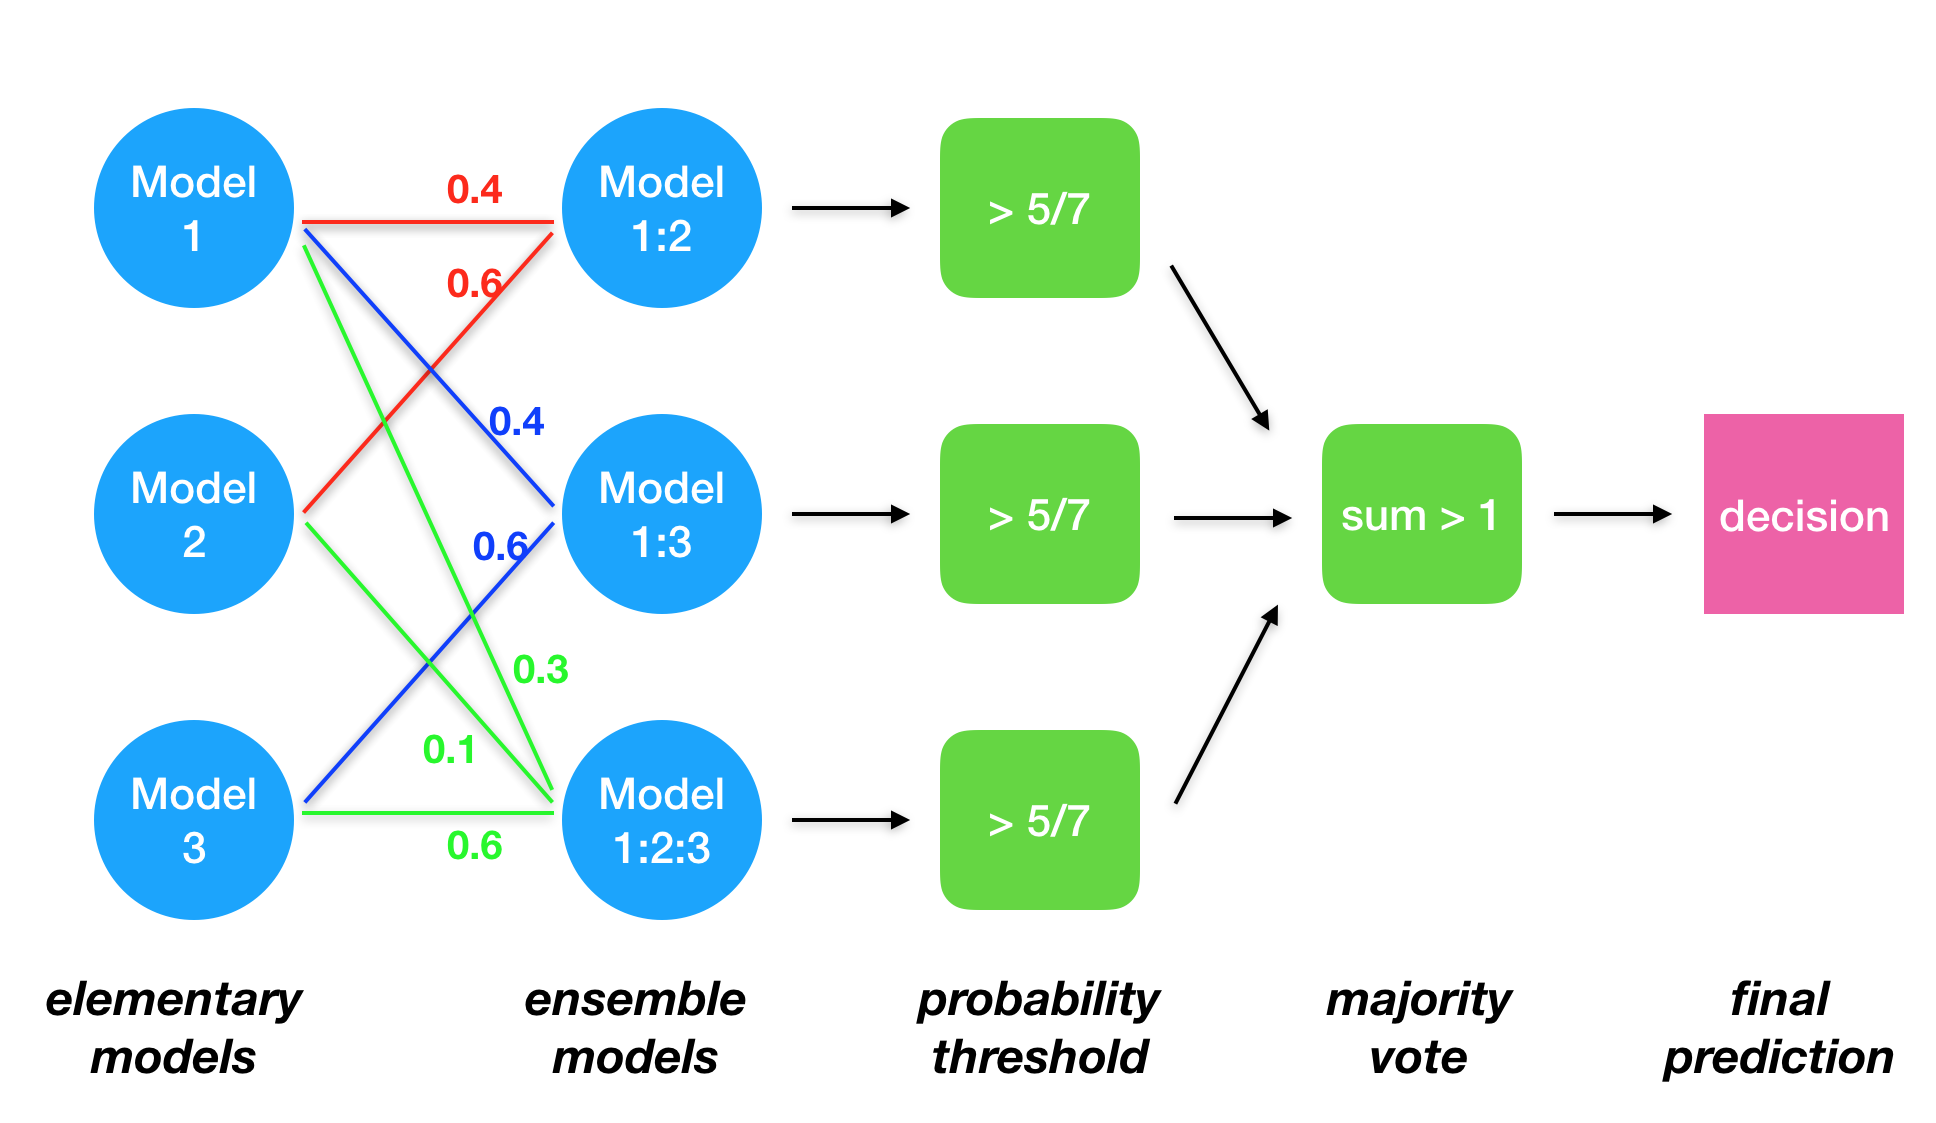
\includegraphics[width = 0.95\textwidth]{figure/Ensemble1.png}
	\end{figure}	

\end{frame}








\begin{frame}
\frametitle{Logistic Ensemble CV Results}

	\begin{figure}[H]
		\centering
		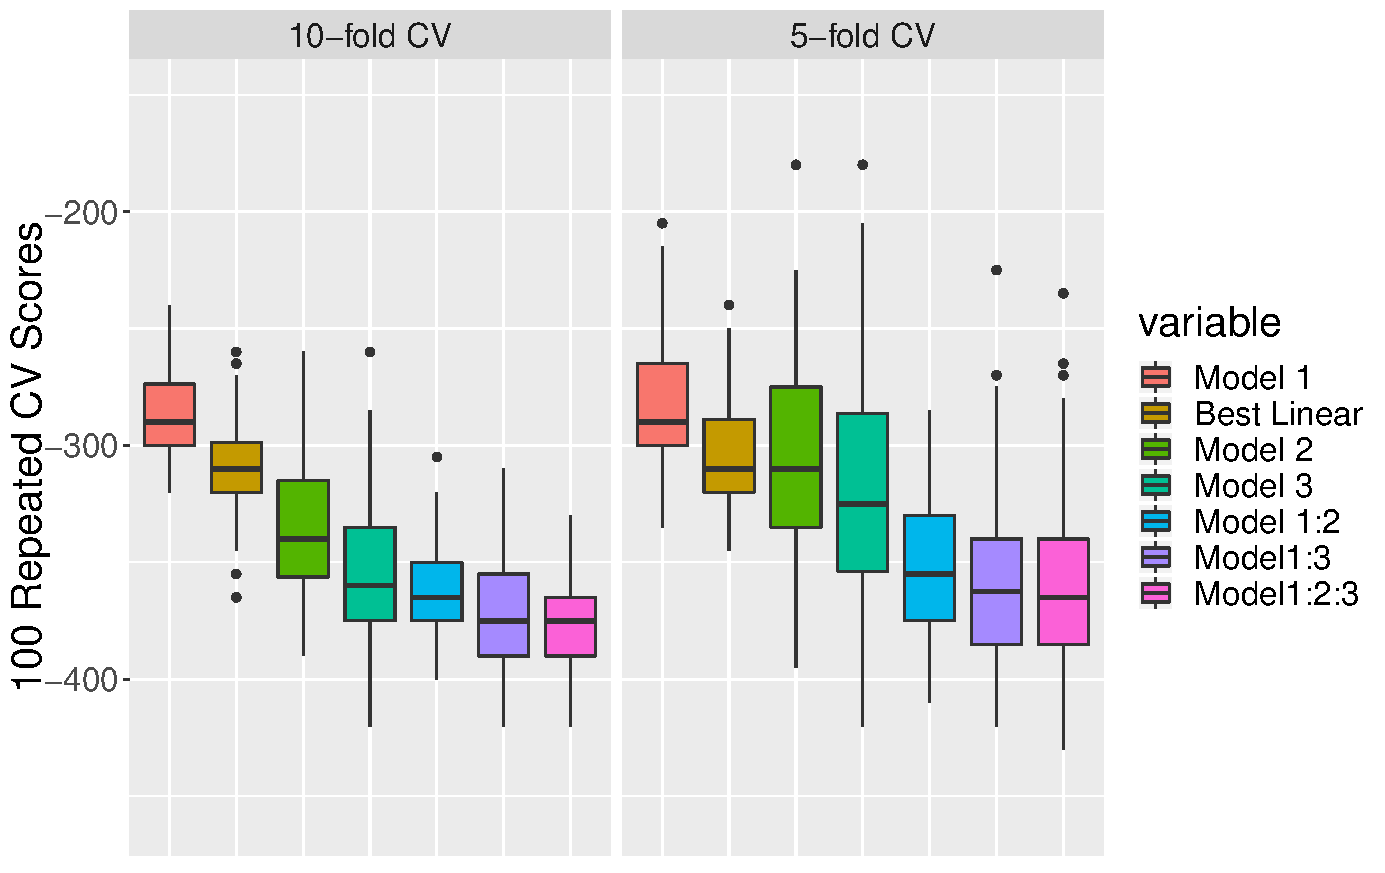
\includegraphics[width = 0.9\textwidth]{figure/logis_ens_result.pdf}
	\end{figure}	

\end{frame}



\begin{frame}
\frametitle{Our Final Solution vs Rest of Top 50 Teams}

	\begin{figure}[H]
		\centering
		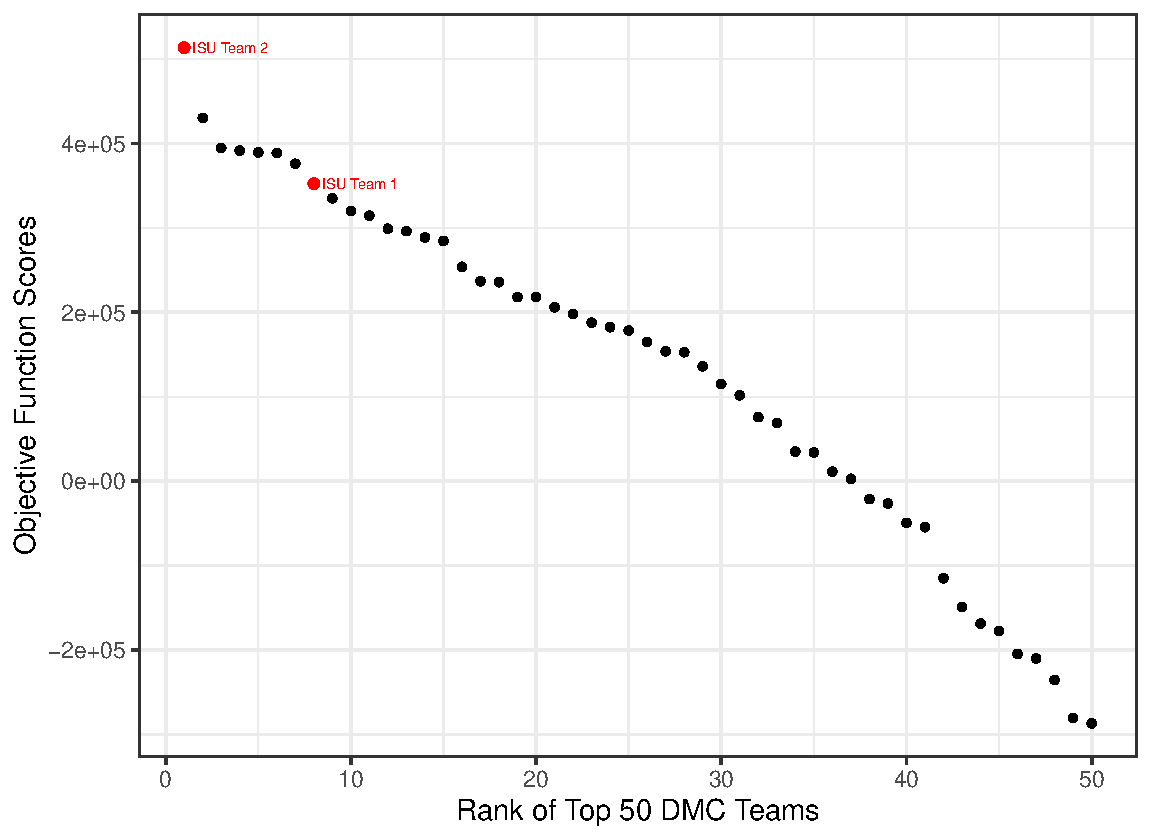
\includegraphics[width = 0.9\textwidth]{figure/rank_top_50.pdf}
	\end{figure}	

\end{frame}



\begin{frame}
\frametitle{All of Our Solutions vs Rest of 2nd Best Team}

	\begin{figure}[H]
		\centering
		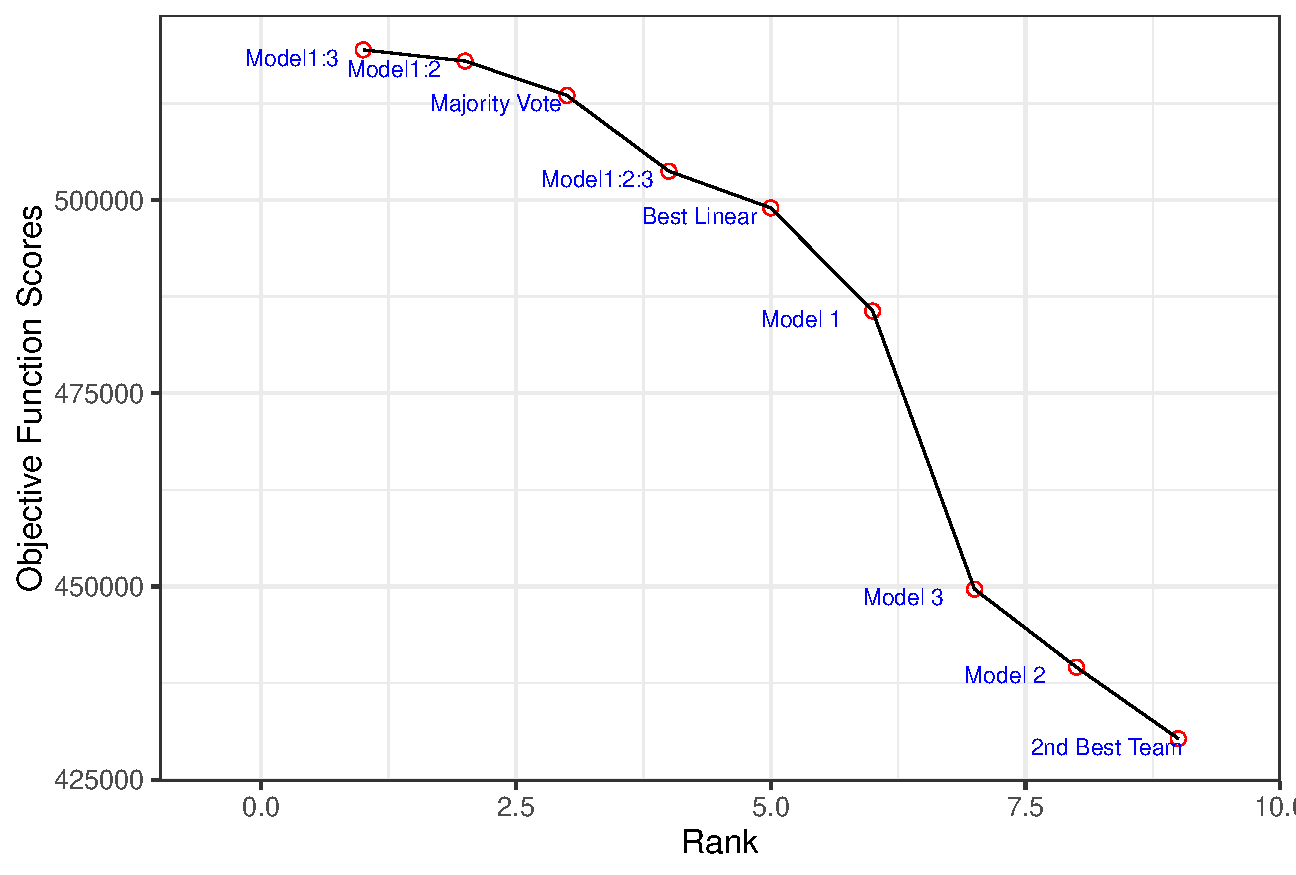
\includegraphics[width = 0.9\textwidth]{figure/rank_our_models.pdf}
	\end{figure}	

\end{frame}




%%%%%%%%%%%%%%%%%%%%%%%%%%%%%%%%%%
\section{Summary}

\begin{frame}
\frametitle{Key Ingredients Lead Us to Win}

\begin{itemize}
\item Derive optimal threshold for unbalanced 2-class loss function.
\item Use multiple evaluation criteria for model selection.
\item Successful feature engineering.
\item Use proper model ensemble method.
\item Most importantly: we do not \textcolor{blue}{overfit} the data.
\end{itemize}

\end{frame}



\begin{frame}
\frametitle{What We Learned from the Contest}

\begin{itemize}
\item Simple models are more preferable for small datasets.
\item Try to use a smaller fold Cross-Validation for a problem with small dataset.
\item Fancy ML/DL methods do not guarantee you to win a data mining contest, spend more time on data.
\end{itemize}

\end{frame}




\begin{frame}
\frametitle{Advice for the Coming Year DMC}

\begin{itemize}
\item Comprehend the task before going through the model details.
\item  Spend more time on data pre-study and feature engineering.
\item Be organized (solve the problem step by step).
\item Team work ( exchanging ideas and thoughts / time arrangement / managing file platform / responsible for teammates ) leads to win the contest.
\item We believe you will have a good performance in the next year's contest as we did.
\end{itemize}

\end{frame}




\begin{frame}%%     1
\begin{center}
\Huge Thank You!
\end{center}
\end{frame}




\end{document}


